\subsection{Experimental Methodology}
In order to carry out our experiments we mainly used the caret(classification and regression training) R package\cite{caret}. 
The function train() from the above package allow us to build a model based on tuning parameter process. 
The tuning of the parameters is performed by cross validation, in particular is a repeated Cross Validation of type 3x5-folds. For each parameter the automated tuning parameter try 5 different values, it means that if the model has p parameters the number of combination it'll try are $5^p$. Based on the maximum Accuracy obtained for each combination it'll pick the set of best parameters.
Once found the needed parameters it builds the model to use for prediction. What we evaluate at the end is the general accuracy of the classification task.

We focused on SVM classifiers in 3 different setup: 
\begin{enumerate}
    \item Simple SVM - Linear kernel
    \item Kernelized SVM - Polynomial kernel
    \item Kernelized SVM - RBF kernel
\end{enumerate}

When passing to train() function of caret package the names "svmLinear", "svmPoly", "svmRadial" we are calling the SVM implementation of the R package $kernlab$\cite{Kernelab}. 
The parameters found with cross validation are:
\begin{enumerate}
    \item For linear kernel: C cost of constraint violation
    \item For polynomial kernel : degree of the polynomial, C cost of constraint violation and scale
    \item For RBF kernel : $\gamma$ parameter and C cost of constraint violation
\end{enumerate}
The values of train and test set are scaled, before modelling process

\subsection{Experiment 1 - Optimal HOG Parameters}
As explained in the \textit{Theory section}[\ref{section:theory}] HOG has two parameters to be tuned:
\begin{itemize}
    \item Number of splits -  number of image partitions.
    \item Number of bins - size of the histogram
\end{itemize}

Let's try to get an intuition on how these parameters will affect the performance. If we just use 1 split, we will be taking the image as a whole. The more splits, the more partitions of the image we will have. If we consider the image as a whole, we will achieve in variance with respect to translations, rotations. However, we will loose the ability to get more grained knowledge, meaning that local part of the image that could be very informative in terms of identifications will be lost when taken together with the rest of the image.
On the other side, if we make a lots of splits in an image, the image will be less invariant to translations or rotations, but each split will allow to capture better the details of that part of the image. So in summary, we would say that the optimal number of splits depends highly on the kind of images. 
Regarding the number of bins, the effect is similar to that of the number of bins. Less umber of bins will make classification more robust to rotations, but at the cost of losing some details that can be important in terms of recognizing the image. 

In this experiment, we will try several combinations of splits and bins, in order to see if there is any combination or values that do provide significant better accuracy. 

The parameters of this experiment are:
\begin{enumerate}
    \item Number of splits = 2, 5, 8, 11, 14, 17
    \item Number of bins = 6, 10, 14, 18, 22.
    \item Number of images per category = 70
    \item Number of classes = 10
    \item Kernel = Linear, Radial. 
\end{enumerate}

The results are the following:

\begin{figure}[H]
    \centering\begin{subfigure}[H]{0.49\linewidth}
    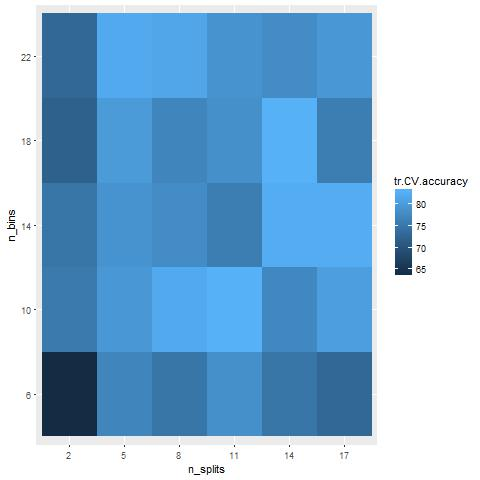
\includegraphics[width=\textwidth]{Images/Accuracy_for_categories_starfish_minaret.jpeg}
    \caption{Linear Kernel}
    \label{subfig:linear}
    \end{subfigure}
    \centering\begin{subfigure}[H]{0.49\linewidth}
    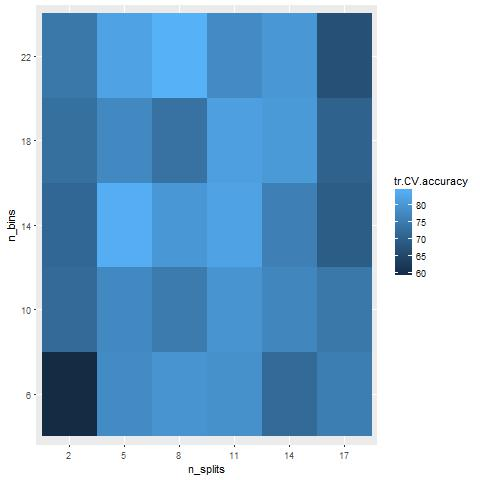
\includegraphics[width=\textwidth]{Images/Accuracy_for_categories_starfish_minaret_radial.jpeg}
    \caption{Radial kernel}
    \label{subfig:radial}
    \end{subfigure}
    \caption{Accuracy results for different HOG parameters}
    \label{fig:exp1}
\end{figure}

The conclusions that we can draw from the above results are the following. From one side, 2 splits seems to be too few, meaning that if we split the image in 4 pieces, we do not have enough specific information about concrete part of the image that are important. However, from 5 to 17 splits, there is no evidence of improvement or deterioration of the accuracy. This would mean that with the given images, if we split the image in 25 parts, we have enough details in order to have information about important parts of the image. On the other side, the fact that having a the image split in 17*17 parts does not deteriorate the performance, means that we should not find a lot of translations and rotations or objects of different sizes in the images. If we explore a bit the dataset, we will see that this is generally true: 


\begin{figure}[H]
    \centering
    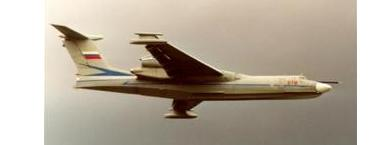
\includegraphics[width=0.3\textwidth]{Images/airplane_1.jpg}
    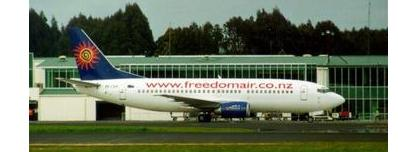
\includegraphics[width=0.3\textwidth]{Images/airplane_2.jpg}
    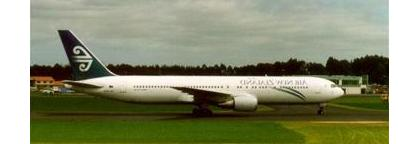
\includegraphics[width=0.3\textwidth]{Images/airplane_3.jpg}
    \caption{Airplane category}
    \label{fig:airplane}
\end{figure}

\begin{figure}[H]
    \centering
    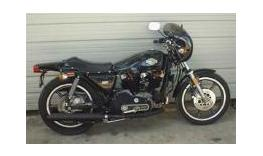
\includegraphics[width=0.3\textwidth]{Images/moto1.jpg}
    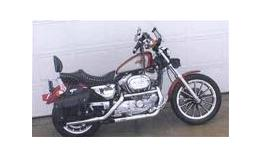
\includegraphics[width=0.3\textwidth]{Images/moto2.jpg}
    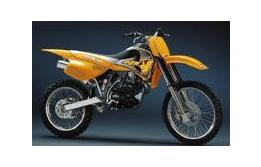
\includegraphics[width=0.3\textwidth]{Images/moto3.jpg}
    \caption{Motorbikes category}
    \label{fig:moto}
\end{figure}

Finally, comparing the results of the linear kernel and the radial kernel, we can see that there are no significant differences. The only thing we see is that with 17 splits, the accuracy in the radial kernel decreases. This may be due to the fact that as radial kernel is able to fit perfectly the data and thus, if we have a very high dimensional feature space, like with 17 splits and 22 bins (17*17*22 = 6538 dimensions), the radial kernel may be over fitting the data. 


In the next experiment, we will see explore if by combining 2 HOG, each of them with different number of binds and different number of splits provides any improvement in the accuracy obtained. 

\subsection{Experiment 2 - Two HOGs Features vector}
After exploring different combinations of $split\times bin\_size$ we wanted to explore the possibilities of creating features vector the comprised from two HOGs. For our experiment, we used the the following setting:

The parameters of this experiment are:
\begin{enumerate}
    \item $HOG_1$ parameters combination = \{4\_6, 6\_6, 8\_6 , 4\_12, 6\_12, 8\_12\}
    \item $HOG_2$ parameters combination = \{10\_6, 12\_6, 14\_6, 16\_6, 10\_12, 12\_12, 14\_12, 16\_12\}
    \item Number of images per category = 70
    \item Number of classes = 10
    \item Kernel = Linear 
\end{enumerate}

We created different features vector combinations by concatenate $HOG_1$ and $HOG_2$ into one features vector, for example, $Features\_vector_{HOG_{11},HOG_{21}} = ((4\_6), (10\_6))$, later we used the "Linear Kernel" to check the performance of the different combination. In figure[\ref{fig:exp1a}] we can see the performance of our classifier. The numbers the axis stands for hog configuration ($HOG(Split\_Bins)$) and the gradient of color stands for the accuracy(\textbf{Note}: the darker blue, the better accuracy). 

\begin{figure}[!h]
    \centering
    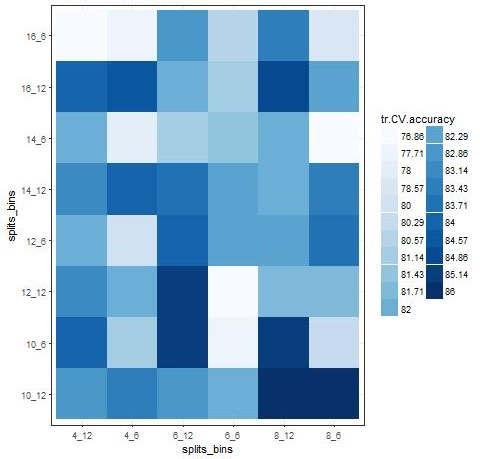
\includegraphics[width=0.6\textwidth]{Images/Accuracy_for_categories_1a.jpeg}
    \caption{Accuracy of Split and Bin combination with linear kernel}
    \label{fig:exp1a}
\end{figure}

From figure[\ref{fig:exp1a}] we can learn, again, that it's hard to draw conclusions for the "right" combination.
\begin{itemize}
    \item Two combinations get 86\% accuracy: $F_1: (8\_6, 10\_12)$ and $F_2: (8\_12,10\_12)$
    \item Three combination get 85.14\% accuracy: $F_3:(6\_12, 10\_6)$, $F_4:(8\_12, 10\_6)$ and \\ $F_5:(6\_12, 12\_12)$
\end{itemize}

Our intuition from the experiment is that HOG with big bin (=12) will be work better with both small and big bin. In case HOG with big bin combined with Hog with small bin, the small bin should have relative high split. This intuition can be used only as \textit{rule of thumb} as we can see, for example, the combination of $HOG(14\_12)$ with $HOG(8\_6)$ perform better than with $HOG(6\_8)$, however, the combination with $HOG(4\_6)$ outperform the bigger split.

The conclusion from the experiment is that in order to get better quality features vector combination we need to apply more complicated technique such as "Spatial Pyramid Matching" as suggested in \cite{Spatial_Pyramid}. Since extending the features vector is costly in power computing (for our poor laptops) and the performance just slightly improved, we decided to stick with one HOG as features vector.

\subsection{Experiment 3 - Dynamically Grows Dataset By Adding Classes}

This experiment is conducted with the aim of understating what is the behavior/performance of each classifier in a dataset that grows dynamically. It means that each classifier is tested first in a dataset of just 2 classes (binary classification) and at each step we will add 1 more class to the dataset in order to check not only the classifier performance over the whole dataset but also the performance of each classifier  with respect to a single class. 
The parameters of this experiment are:
\begin{enumerate}
    \item Number of splits = 4
    \item Number of bins = 15
    \item Number of images per category = 70
    \item Number of classes = 10
\end{enumerate}
Each feature descriptor vector will have length $4\times4\times15 = 240$, 700 images in total.\\

% left minipage%
\begin{minipage}{0.45\textwidth}

\begin{table}[H]
\scalebox{0.8}{
\begin{tabular}{|l|l|l|l|}
\hline
\textit{Sensitivity}        & Linear        & Polynomial        & RBF         \\ \hline
\rowcolor[HTML]{FFFC9E} 
2. Starfish *               & 0,77          & 0.61              & 0.72        \\ \hline
2. Minaret *                & 1             & 0.94              & 1           \\ \hline
\rowcolor[HTML]{FFFC9E} 
3. Bonsai                   & 0.94          & 0.77              & 0,72        \\ \hline
\rowcolor[HTML]{FFFC9E} 
4. Scorpion                 & 0.44          & 0.66              & 0.44        \\ \hline
5. Motorbikes               & 1             & 1                 & 1           \\ \hline
\rowcolor[HTML]{FFFC9E} 
6. Faces                    & 1             & 0.94              & 0.88        \\ \hline
7. Watch                    & 0.83          & 0.83              & 0.83        \\ \hline
7. Airplanes                & 0.94          & 1                 & 1           \\ \hline
9. Umbrella                 & 0,88          & 0,83              & 0.83        \\ \hline
10. Trilobite               & 1             & 1                 & 1           \\ \hline
\multicolumn{4}{|l|}{* These to classes are the first used in the first step} \\ \hline
\end{tabular}
}
\caption{Sensitivity over classifiers}
\label{table:sens}
\end{table}

\end{minipage}
%right minipage%
\begin{minipage}{0.55\textwidth}
\begin{figure}[H]
\centering
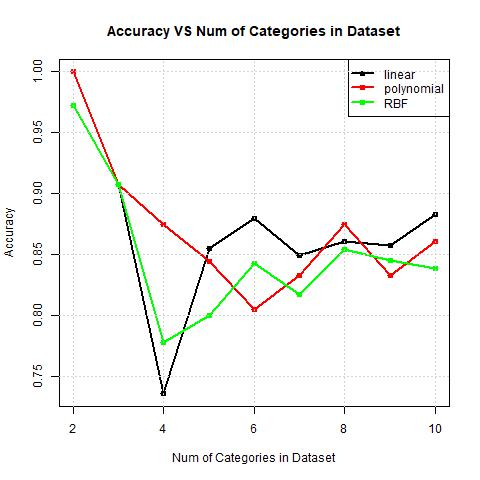
\includegraphics[width=0.9\textwidth]{Images/Number_categories_vs_accuracystarfish_minaret.jpeg}
\caption{Accuracy VS Num Categories}
\label{fig:exp3}
\end{figure}
\end{minipage}

Checking the results above(Table[\ref{table:sens}], Figure[\ref{fig:exp3}]) we can see that generally a linear kernel perform better than the others, sometimes gaining a gap greater than a 20\%. Interesting is the behavior of the classifiers in the class $4. Scorpion$. It seems a complicated class to understand, a class where RBF and linear SVM fail completely (even going under 0.5 of sensitivity) while the polynomial manage to do something better catching a 0.66 in sensitivity (however still an overall low value compared with the other class).

\subsection{Experiment 4 - Kernels Function Comparison}

In this section, we will compare the performance of the SVM with several different kernel functions. In theory, if the 10 classes are not linearly separable, we should see an increase of performance when using RBF kernel or Polynomial Kernel instead of Linear Kernel. However, after having run experiments up to now, we have not seen such behaviour. anyways let's set up an experiment to check it. In this case, as we want to enforce full classes separability, we will not use \textit{caret} to train the SVM, but we will force the parameter C to 100 to penalize the miss-classification errors and ensure full separability. We will also try different number of images to see if there is any dependency on the training size for any kernel. 

\begin{enumerate}
    \item Number of splits = 4
    \item Number of bins = 15
    \item Number of images per category = 15, 30, 45, 60, 70
    \item Cost = 100
    \item Number of classes = 10
    \item Kernels = Linear, Polynomial 2, Polynomial 3, RBF, LaplacianRBF.  
\end{enumerate}

The results are the following.

\begin{figure}[H]
\centering
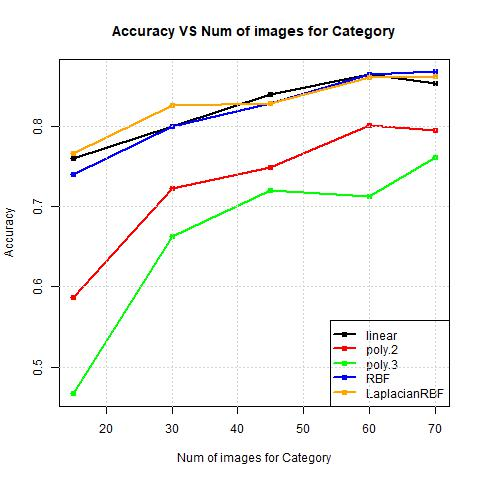
\includegraphics[width=0.7\textwidth]{Images/Kernel Methods.jpeg}
\caption{Accuracy for different kernel functions}
\end{figure}

As we can see, the thee linear, RBF and Laplacian RBF kernel functions have very similar performance for all training data sets sizes used. Considering that we have set C parameter to 100 and we have leaved the sigma parameter to default, the fact that we have similar performance with radial kernels and linear kernels tells us that there is a linear classifier that gives full separability of the data, in the feature space dimensions we are working at. Thus, there is no need for non-linear feature space transformations provided by the radial kernel functions. We will discuss more in depth this point in the conclusions. 


\subsection{Experiment 5 - Comparison With Traditional Methods}

As mentioned in the introduction, SVM are expected to have a better generalization performance with problems in high dimensional spaces than traditional methods. In this experiment we will compare the performance of the following methods: Naive Bayes, Classification Tree, LDA, KNN. All of them will be trained automatically using Caret Package, and compared with a SVM with both Linear Kernel and RBF kernel. 

\begin{enumerate}
    \item Number of splits = 4
    \item Number of bins = 15
    \item Number of images per category = 15
    \item Number of classes = 10
\end{enumerate}

The results are the following:

\begin{figure}[H]
\centering
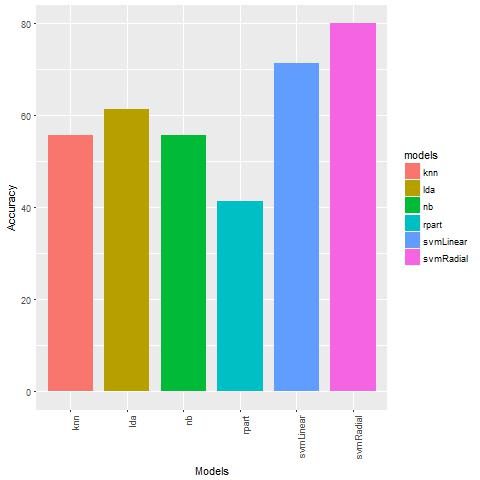
\includegraphics[width=0.7\textwidth]{Images/Accuracy_for_categories_starfish_minaret_2.jpeg}
\caption{Accuracy for different methods}
\end{figure}

As we can see, SVM outperforms the other methods, by at least 10 percent. However, here we have used only 15 images. It would be interesting to see the evolution if we use more data to train the methods. 

Next, we will execute all 6 models with different number of images, to see how the differences change when adding different number of images:

\begin{enumerate}
    \item Number of splits = 4
    \item Number of bins = 15, 30, 45, 60, 70
    \item Number of images per category = 15
    \item Number of classes = 10
\end{enumerate}

The results are the following:

\begin{figure}[H]
\centering
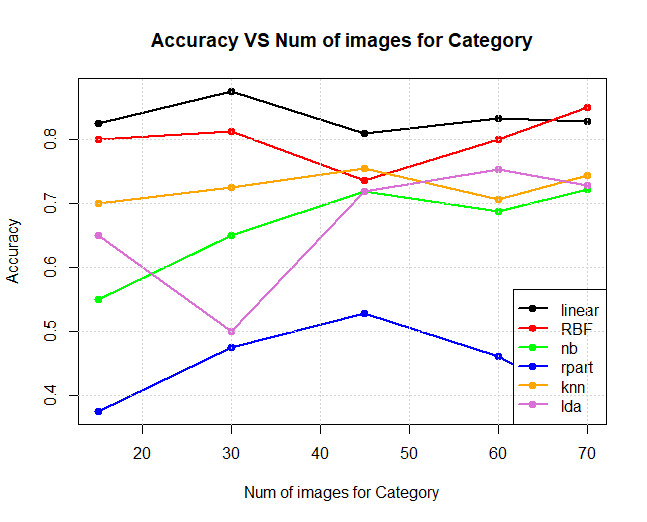
\includegraphics[width=0.6\textwidth]{Images/WhatsApp.jpeg}
\caption{Accuracy vs num category by method}
\end{figure}

As we saw in the previous plot, with 15 images, the SVM with 80 \% accuracy methods have at least 10 accuracy points more than next method which is KNN with 70 \%, while other methods range from 37\% for classification tree to 65\% of linear discriminant. While increasing the number of images, we see that methods like the Naive Bayes or the Linear discriminant get up to 70 \% of accuracy, same as KNN but none of them reaches the 80\% of the support vector machines. Thus, we confirm that even with little data, the generalization performance of the support vectors is much better, as it is more robust to outliers or any other points that may appear when adding more data. As expected, the generalization performance of other methods improves with more data (except with the classification tree), but does not reach the accuracy obtained with SVM even with much less data. 

\subsection{Experiment 6 - Dynamically Grows Classes in Dataset} \label{experiment_6}
In this experiment we want to investigate what happens when we increase the number of images, once fixed the number of categories and the parameters to build the HOG for each image. 
The steps chosen to perform this task are 15, 30, 45, 60, 70. We stop at 70 because there are categories with no more than 70 photos.
The other parameters are set to the following values:
\begin{enumerate}
    \item Number of splits = 4
    \item Number of bins = 15
    \item Number of classes = 10
    \item Classes :  Bonsai, Motorbikes, Scorpion, Faces,  Umbrella, Airplanes, Trilobite, Watch, Starfish, Minaret
\end{enumerate}

The aim of this experiment is to check if there is any relation between the number of images in the dataset to classify and the classifier (kernelized, not kernelized, etc..)

\begin{figure}[H]
\centering
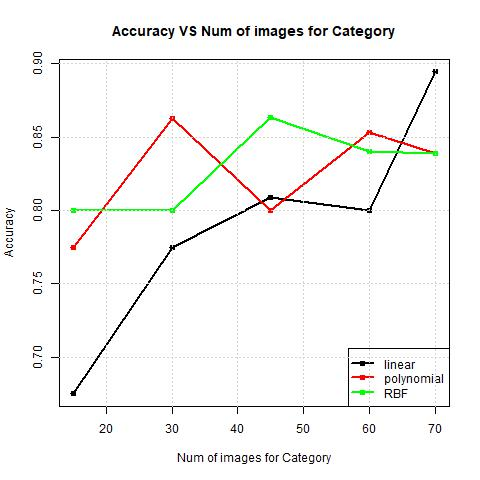
\includegraphics[width=0.6\textwidth]{Images/Accuracy_for_categories_bonsai_Motorbikes.jpeg}
\caption{Accuracy VS Num Images}
\end{figure}

Looking at the plot we can't state an exact conclusion, we are aware that the number of images may be low so actually we don't know what happens when the images are like 150 per category. Generally we can only state that the trend is positive for all the classifier, all of them increase the accuracy increasing the number of images fed into the classifier. 